\documentclass[leqno, b5paper]{khalid-urdu-book}
\begin{document}
\باب{طبیعیات} %chapter
\حصہ{پیمائش} %Section
اس کتاب کے پہلے باب کا پہلا حصہ ہے۔

\جزوحصہ{ا ب ج} %Subsection
وغیرہ وغیرہ

\جزوجزوحصہ{ا ب ج} %subsubsection

\جزوجزوحصہ{ا ب ج} %subsubsection

\جزوحصہ{ا ب ج} %subsection

\حصہ{ا ب ج} %section

\begin{table}[h!]
	\centering
	\begin{tabular}{|c|c|c c|} %Columns
		\hline % hline means single horozontal line  
		ا ب ج & ا ب ج & ا ب ج & ا ب ج\\ %"\\" for next line
		\hline\hline
		ا ب ج & ا ب ج & ا ب ج & ا ب ج\\
		\hline
		ا ب ج & ا ب ج & ا ب ج & ا ب ج\\
		\hline
	\end{tabular}
\caption{جدول کا نام} % Table's name
\label{tab:my_label}
\end{table}

\begin{align} %eqautions with numbering
	(a+b)^{2} &= a^{2}+2ab+b^{2}\\ % "&" used to align equals to
	(a-b)^{2} &= a^{2}-2ab+b^{2}\\
	\SI{24}{\meter\per\second} &= \SI{26}{\newton\meter\squared}\\
	%SI is used for uints 
	\SI{5e24}{\meter\cubed} &= \SI{9e-32}{\meter\tothe{10}}
	% e is used for  x10   
\end{align}
\begin{figure}
	\centering
	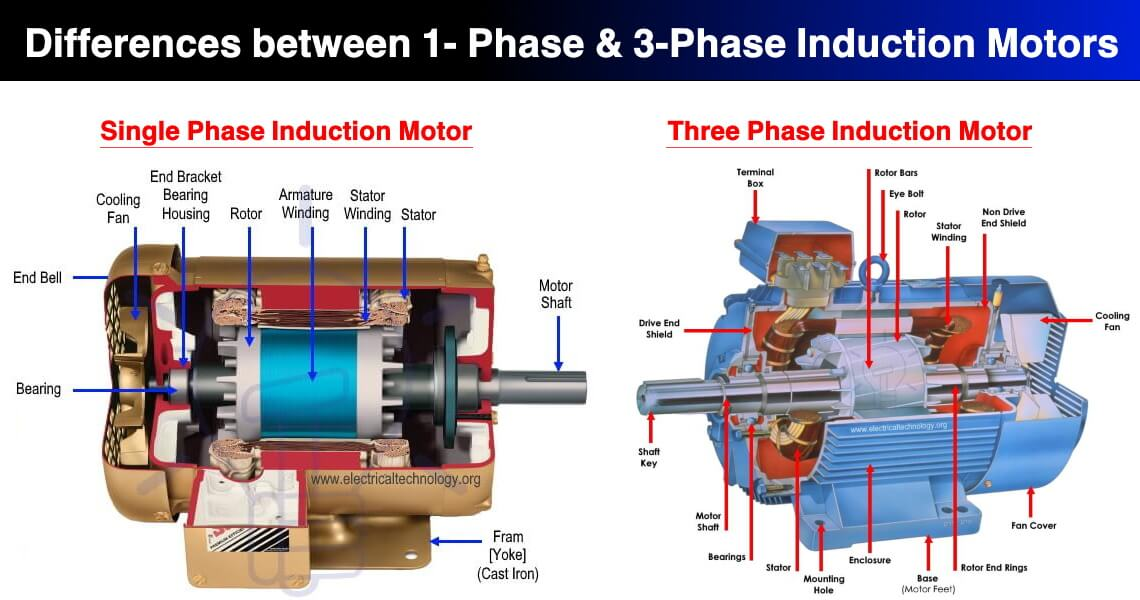
\includegraphics[width=\linewidth]{Induction Motor}
	\caption{امالی موٹر}
	\label{for reference}
\end{figure}



\end{document}

